\section{\texorpdfstring{Tổng quan các công trình nghiên cứu liên quan}{Content}}
Việc tạo sinh dữ liệu mới trong thời gian gần đây đã phát triển mạnh mẽ với sự ra đời của kiến trúc mạng GANs. Hệ thống mạng GANs bao gồm các mạng học máy, học sâu nhỏ hơn, chia thành hai thành phân là mạng tạo sinh dữ liệu (mạng G) và mạng phân biệt dữ liệu (mạng D). Mạng G đóng vai trò như khối Decoder trong bộ Variational Autoencoder \cite{vae_base},  có chức năng học và xấp xỉ được phân phối xác suất của dữ liệu gốc, từ đó tạo sinh ra dữ liệu mới giữ được đặc trưng và tương đồng với dữ liệu gốc. Mạng D có chức năng phân biệt giữa dữ liệu được tạo sinh bởi mạng G và tập dữ liệu huấn luyện. Trong quá trình huấn luyện, dựa trên hàm mất mát của D, các trọng số của cả hai mạng G và D đều được cập nhật trong quá trình lan truyền ngược, từ đó giúp hai mạng này tăng độ chính xác. Với mạng G, qua quá trình huấn luyện, mạng sẽ có khả năng tạo sinh ra được dữ liệu ngày càng chân thực hơn, khó phân biệt hơn. Trong khi đó, mạng D cũng ngày càng có chức năng phân biệt tốt hơn, chuẩn xác hơn. Đến một lúc nào đó, độ chính xác của hai mạng sẽ đạt đến mức cân bằng, lúc này hai mạng đã hội tụ và không thể được cải thiện hơn với kiến trúc mạng và tập dữ liệu huấn luyện hiện tại, nên ta sẽ dừng quá trình huấn luyện tại đây.

%------------------------------------------------------------------------

\subsection{\texorpdfstring{Bài nghiên cứu "Lip Movements Generation at a Glance"\cite{chen2018}}{Target}}

\begin{figure}[H]
    \centering
    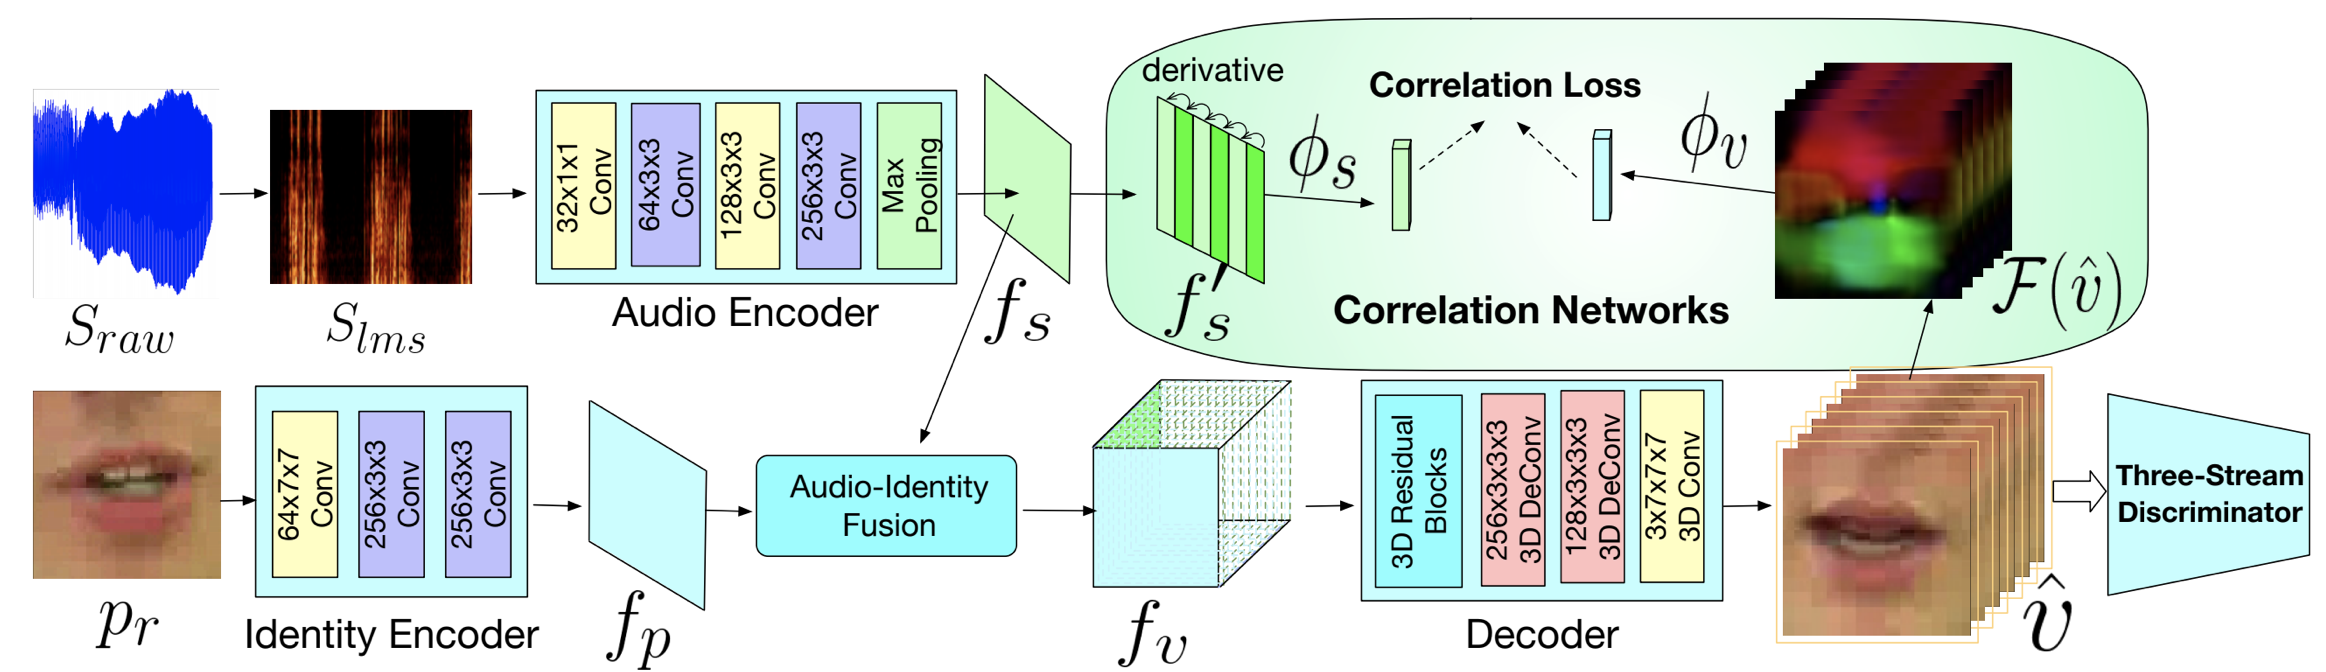
\includegraphics[width=15cm]{./content/images/chen2018_model.png}
    \caption{Mô hình của bài báo Lip Movements Generation at a Glance}
    \label{fig:chen2018_model}
\end{figure}

Việc tạo sinh khẩu hình miệng khớp với tiếng nói là bước đầu tiên để thực hiện việc tạo sinh khuôn mặt. Nghiên cứu này đã thành công trong việc tạo sinh khẩu hình miệng từ một ảnh tĩnh chứa hình ảnh khuôn miệng của một người bất kỳ, và một đoạn âm thanh chứa tiếng nói. Bằng phương pháp kết hợp các đặc trưng âm thanh và hình ảnh, nghiên cứu cho ra kết quả tốt và có độ chính xác cao hơn so với các nghiên cứu trước đó. Hình \ref{fig:chen2018_model} mô tả cấu trúc của mạng tạo sinh ảnh được dùng. Đầu tiên, âm thanh được cắt thành các đoạn nhỏ dài 0.64s, các đoạn này được chuyển thành phổ Log-Mel ($S_{raw}$ thành $S_{lms}$), sau đó qua một bộ Audio Encoder để trích đặc trưng, ta có đặc trưng âm thanh $f_s$ là một ma trận 2 chiều kích thước $F \times T$. Bên cạnh đó, hình ảnh khuôn miệng cũng được đưa qua một bộ Identity Encoder để tạo thành ma trận 2 chiều $f_p$ kich thước $H \times W$.

\begin{figure}[H]
    \centering
    \begin{minipage}{0.48\textwidth}
        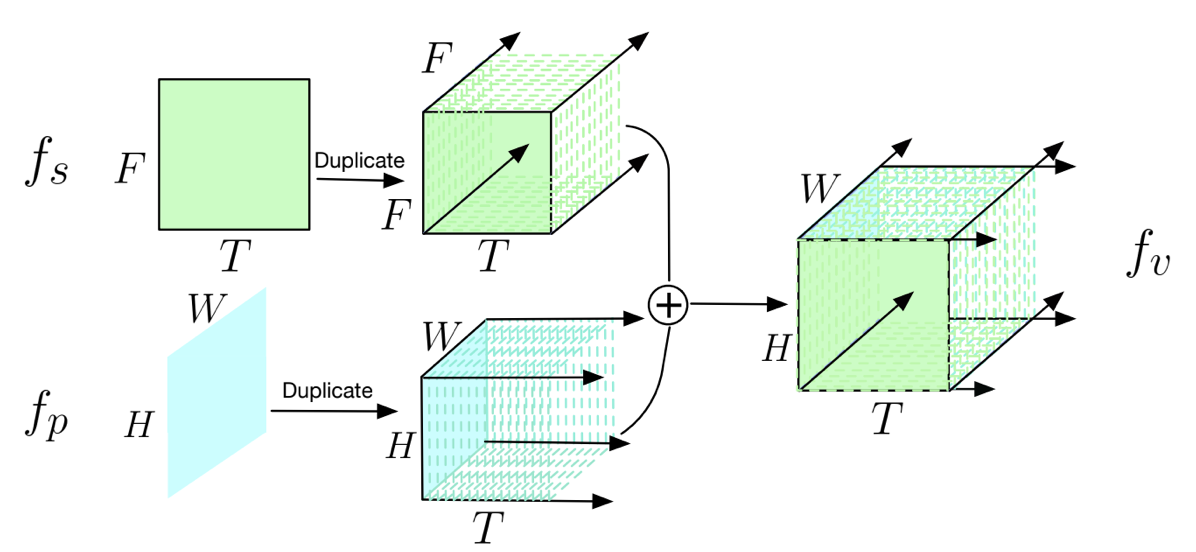
\includegraphics[width=7cm]{./content/images/chen2018_fusion.png}
        \caption{Phương pháp kết hợp đặc trưng hình ảnh và âm thanh}
        \label{fig:chen2018_fusion}
    \end{minipage}\hfill
    \begin{minipage}{0.48\textwidth}
        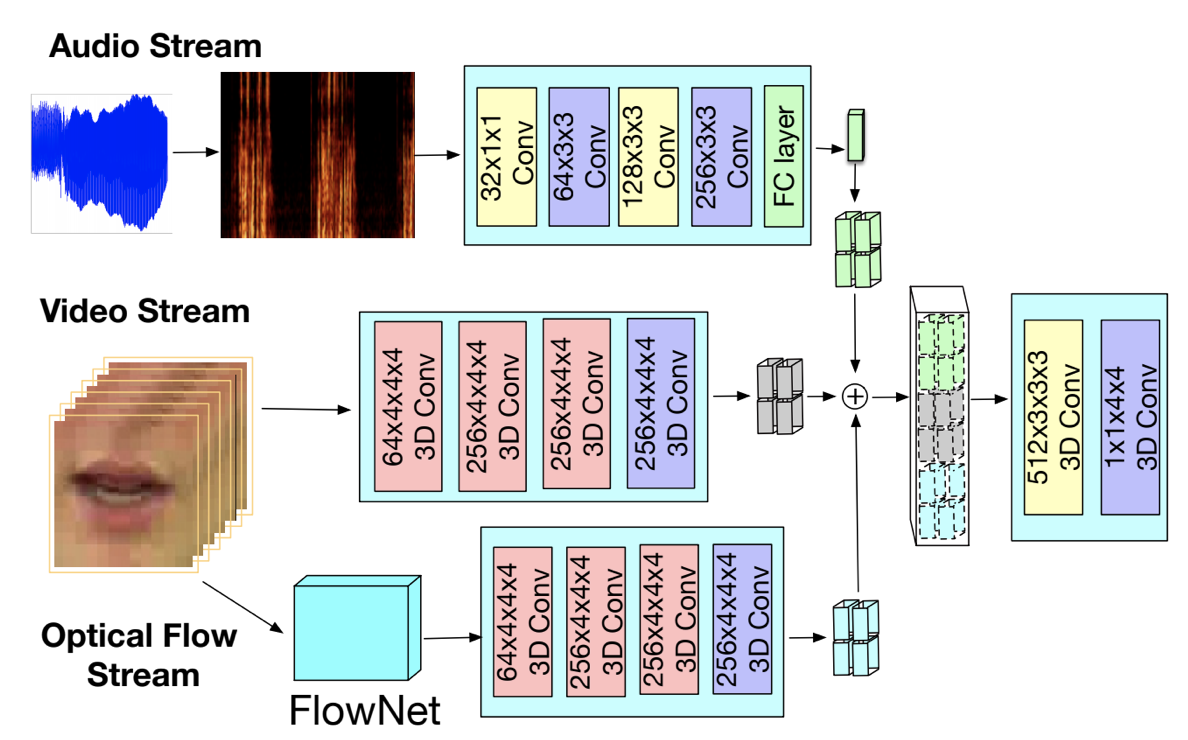
\includegraphics[width=7cm]{./content/images/chen2018_gans.png}
        \caption{GANs Discriminator với 3 loại đặc trưng}
        \label{fig:chen2018_gans}
    \end{minipage}
\end{figure}

Để kết hợp hai đặc trưng hình ảnh, âm thanh với nhau để tạo sinh hình ảnh mới, tác giả bài báo đề xuất phương pháp nhân bản ma trận $f_s$ F lần và nhân bản ma trận $f_p$ T lần thành hai tensor ba chiều, sau đó nối tiếp các kênh của hai tensor này để tạo thành khối tensor ba chiều mới. Để có thể nối tiếp được với nhau, Tác giả đã đặt các thông số $H = W = F$. Hình \ref{fig:chen2018_fusion} miêu tả cách kết hợp hai đặc trưng hình ảnh - âm thanh thành khối đặc trưng chung $f_v$, khối $f_v$ có kích thước $W \times H \times T$. Khối đặc trưng này sau cùng được chuyển đổi thành ảnh đầu ra $\hat{v}$ nhờ vào mạng Decoder. Mạng Decoder này sử dụng kiến trúc 3D Residual và các khối Deconvolution nhằm bảo toàn các đặc điểm của hình ảnh gốc.

Đồng thời, nghiên cứu này cũng chỉ ra rằng đặc tính của khuôn miệng trong video là hình ảnh thường đi trước âm thanh, và độ trễ âm thanh - hình ảnh là không đồng nhất trong các video khác nhau. Vì vậy, để tạo sinh một video chân thực, ta phải quan tâm đến độ trễ này. Khối Correlation Network trong hình \ref{fig:chen2018_model} miêu tả cách tính toán giá trị Corellation Loss. Để tính giá trị này, bộ tính toán cần có một encoder ($\phi_s$) để encode sự thay đổi của âm thanh và một encoder ($\phi_v$) để encode sự thay đổi của hình ảnh. Ma trận $f_s$ được tính đạo hàm theo trục T thành $f'_s$, hình ảnh được tạo sinh $\hat{v}$ cũng được đưa qua hàm $\mathcal{F}$ để lấy đặc trưng Optical Flow. Sau đó, cả hai đặc trưng thể hiện sự thay đổi của âm thanh và hình ảnh theo thời gian này được đưa qua các encoder $\phi_s$ và $\phi_v$ để tạo ra hai vector có cùng số chiều.Công thức tính của giá trị Correlation Loss chính là hiệu của 1 và giá trị cosin giữa hai vector đặc trưng cuối cùng:

\begin{equation}
    \ell_{corr} = 1 - \frac{\phi_s(f'_s)\cdot\phi_v(\mathcal{F}(v))}{\|\phi_s(f'_s)\|_2\cdot\|\phi_v(\mathcal{F}(v))\|_2}
    \label{eqn:chen2018_corr_loss}
\end{equation}


Cấu trúc mạng GANs cũng đã được sử dụng trong nghiên cứu này nhằm mục đích tạo ra chuyển động mượt mà cho chuỗi hình ảnh trong video và làm cho chất lượng ảnh tạo sinh tốt hơn. Bộ phân biệt (Discriminator) giữa ảnh thật và ảnh tạo sinh ($D$) được miêu tả trong hình \ref{fig:chen2018_gans}. Đặc trưng Log-Mel của âm thanh được encode thành một vector bằng một mạng Convolution - Fully connected, sau đó vector này được nhân bản và ghép nối để có số chiều bằng với tensor của hai đặc trưng còn lại. Hình ảnh được đưa vào mạng được encode bởi các khối 3D Convolution để có được tensor đặc trưng ảnh. Các ảnh này cũng được đưa qua mạng FlowNet để đưa ra đặc trưng Optical Flow, đặc trưng này cũng được encode để tạo ra tensor đặc trưng cho chuyển động trong video. Sau cùng, ba đặc trưng này được ghép nối tiếp theo kênh và được đưa qua các khối 3D Convolution để lấy được xác suất dự đoán ảnh thật hay tạo sinh của mạng. Cặp video - âm thanh đưa vào mạng có thể là video thật và đoạn âm thanh khớp với video đó, hoặc video thật và một đoạn âm thanh khác, hoặc video được tạo sinh và đoạn âm thanh tương ứng tạo ra nó. Hàm mất mát của mạng được định nghĩa như sau:

\begin{equation}
    \ell_{dis} = -logD([s^j, v^j]) - \lambda_plog(1 - D([s^j, \hat{v}])) - \lambda_ulog(1 - D([s^j, v^k])), k \ne j
\end{equation}

Để so sánh sự tương đồng về mặt tổng quan giữa hai video (video thật và video được tạo sinh), tác giả sử dụng một bộ Autoencoder. Bộ Autoencoder này được huấn luyện độc lập với mạng chính và sử dụng cùng bộ dữ liệu với mạng chính. Phần encoder ($\varphi$) được giữ lại để encode hình ảnh từ video nhằm mục đích trích xuất đặc trưng của chuỗi hình ảnh. Hàm Perceptual Loss $\ell_{perc}(\hat{v}, v)$ được dùng để tính toán độ sai lệch về mặt tổng quan giữa video được tạo sinh từ tiếng nói và video thật tương ứng với tiếng nói:
\begin{equation}
    \ell_{perc}(\hat{v}, v) = \|\varphi(v) - \varphi(\hat{v})\|^2_2
    \label{eqn:chen2018_perc_loss}
\end{equation}

Hàm mất mát của cuối cùng của mạng được định nghĩa:
\begin{equation}
    \mathcal{L} = \ell_{corr} + \lambda_1\ell_{pix} + \lambda_2\ell_{perc} + \lambda_3\ell_{gen}
    \label{eqn:chen2018_loss}
\end{equation}

Trong đó:
\begin{itemize}
\item $\ell_{corr}$: Là giá trị mất mát do sự sai lệch giữa hình ảnh và âm thanh đã nêu ở (\ref{eqn:chen2018_corr_loss}).
\item $\ell_{pix}$: Giá trị mất mát dựa trên sự sai khác ở cấp độ điểm ảnh giữa ảnh được tạo sinh và ảnh trong video thật, $\ell_{pix} = \|v-\hat{v}\|$.
\item $\ell_{perc}$: Giá trị mất mát đo độ sai khác trên toàn bộ chuỗi hình ảnh (đã nêu ở (\ref{eqn:chen2018_perc_loss})).
\item $\ell_{gen}$: Giá trị mất mát của bộ tạo sinh ảnh dựa trên hàm phân biệt $D$: $\ell_{gen} = -logD([s^j, \hat{v}^j])$.
\end{itemize}

Mô hình được huấn luyện và kiểm thử trên các tập dữ liệu GRID, LDC và LRW. Kết quả kiểm thử cho thấy mô hình này cho kết quả tạo sinh hình ảnh tốt hơn hẳn so với các nghiên cứu trước đó. Các độ đo PSNR, SSIM, LMD và CPBD (đã nêu ở phần \ref{sec:metrics_eval}) được sử dụng để kiểm chứng. Sau đây là kết quả được khảo sát bới tác giả:

\begin{figure}[H]
    \centering
    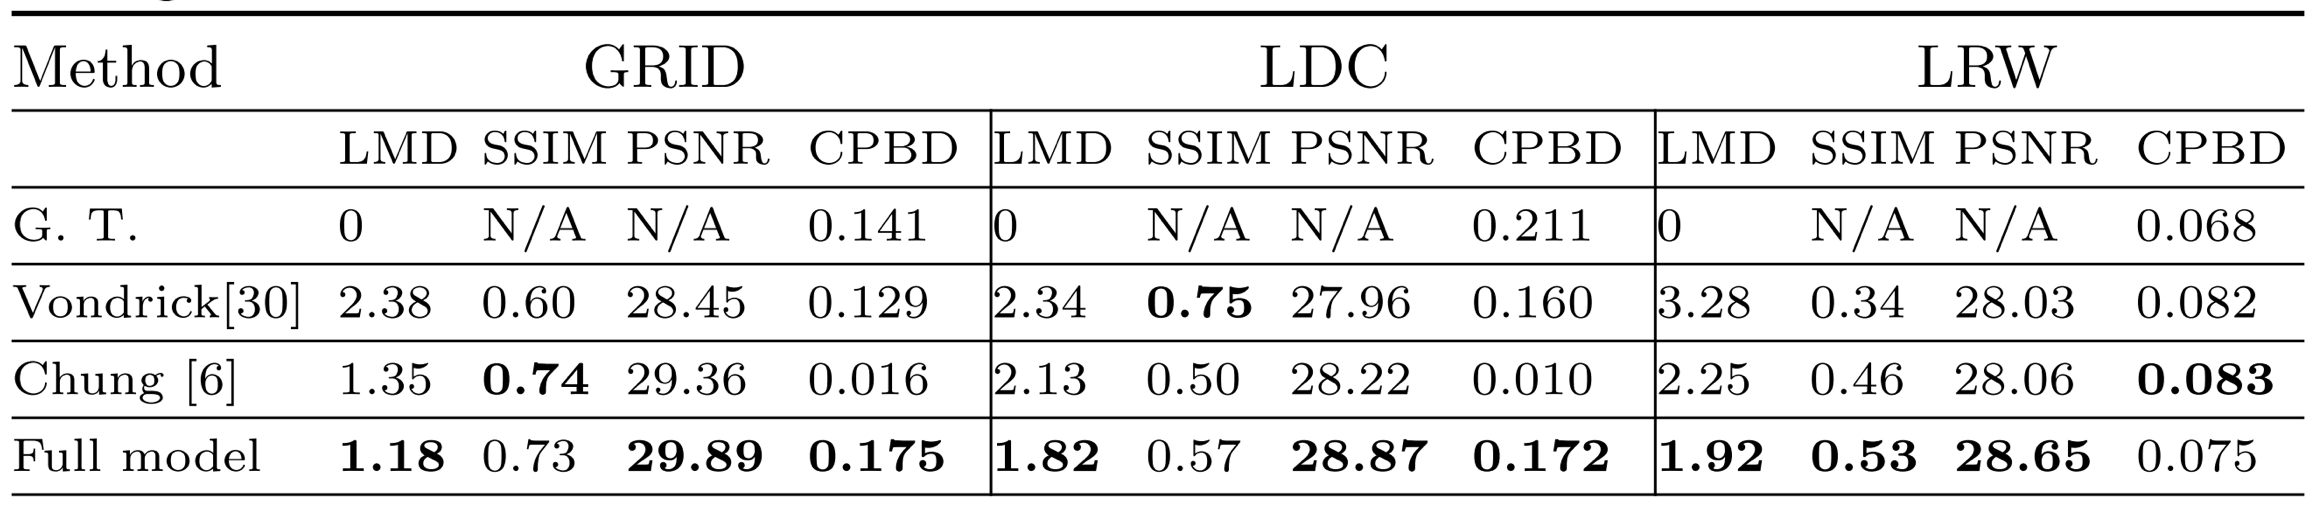
\includegraphics[width=15cm]{./content/images/chen2018_result.png}
    \caption{Kết quả đánh giá và so sánh mô hình trong nghiên cứu Lip Movements Generation at a Glance}
    \label{fig:chen2018_result}
\end{figure}

%------------------------------------------------------------------------

